%%%%%%%%%%%%%%%%%%%%%%%%%%%%%%% beamer %%%%%%%%%%%%%%%%%%%%%%%%%%%%%%%%%%%%%%%%%%%%%%%%%
% To run - pdflatex filename.tex
%      acroread filename.pdf
%%%%%%%%%%%%%%%%%%%%%%%%%%%%%%%%%%%%%%%%%%%%%%%%%%%%%%%%%%%%%%%%%%%%%%%%%%%%%%%%%%%%%%%%

\documentclass[compress,oilve]{beamer}
\mode<presentation>

\usetheme[]{CambridgeUS}
% other themes: AnnArbor, Antibes, Bergen, Berkeley, Berlin, Boadilla, boxes, CambridgeUS, Copenhagen, Darmstadt, default, Dresden, Frankfurt, Goettingen,
% Hannover, Ilmenau, JuanLesPins, Luebeck, Madrid, Maloe, Marburg, Montpellier, PaloAlto, Pittsburg, Rochester, Singapore, Szeged, classic

\usecolortheme{beaver}
% color themes: albatross, beaver, beetle, crane, default, dolphin,  fly, lily, orchid, rose, seagull, seahorse, sidebartab, whale, wolverine

\usefonttheme{professionalfonts}
% font themes: default, professionalfonts, serif, structurebold, structureitalicserif, structuresmallcapsserif


\hypersetup{pdfpagemode=FullScreen} % makes your presentation go automatically to full screen

% define your own colors:
\definecolor{Red}{rgb}{1,0,0}
\definecolor{Blue}{rgb}{0,0,1}
\definecolor{Green}{rgb}{0,1,0}
\definecolor{magenta}{rgb}{1,0,.6}
\definecolor{lightblue}{rgb}{0,.5,1}
\definecolor{lightpurple}{rgb}{0.8, 0.6, 0.9}
\definecolor{gold}{rgb}{.6,.5,0}
\definecolor{orange}{rgb}{1,0.4,0}
\definecolor{hotpink}{rgb}{1,0,0.5}
\definecolor{newcolor2}{rgb}{.5,.3,.5}
\definecolor{newcolor}{rgb}{0,.3,1}
\definecolor{newcolor3}{rgb}{1,0,.35}
\definecolor{darkgreen1}{rgb}{0, .35, 0}
\definecolor{darkgreen}{rgb}{0, .6, 0}
\definecolor{darkred}{rgb}{.75,0,0}
\definecolor{skyblue}{HTML}{75bbfd}

\definecolor{olive}{cmyk}{0.64,0,0.95,0.4}
\definecolor{purpleish}{cmyk}{0.75,0.75,0,0}

% can also choose different themes for the "inside" and "outside"

% \usepackage{beamerinnertheme_______}
% inner themes include circles, default, inmargin, rectangles, rounded

% \usepackage{beamerouterthemesmoothbars}
% outer themes include default, infolines, miniframes, shadow, sidebar, smoothbars, smoothtree, split, tree


\useoutertheme[subsection=true, height=40pt]{smoothbars}

% to have the same footer on all slides
%\setbeamertemplate{footline}[text line]{STUFF HERE!}
\setbeamertemplate{footline}[text line]{} % makes the footer EMPTY
% include packages
%

%show the page numbers in footnote
%\addtobeamertemplate{navigation symbols}{}{%
%	\usebeamerfont{footline}%
%	\usebeamercolor[fg]{footline}%
%	\hspace{1em}%
%	\insertframenumber/\inserttotalframenumber
%}

\setbeamercolor{footline}{fg=purpleish}
\setbeamerfont{footline}{series=\bfseries}

%add color to curent subsection
\setbeamertemplate{section in head/foot}{\hfill\tikz\node[rectangle, fill=darkred, rounded corners=1pt,inner sep=1pt,] {\textcolor{white}{\insertsectionhead}};}
\setbeamertemplate{section in head/foot shaded}{\textcolor{darkred}{\hfill\insertsectionhead}}

% Remove bullet of subsections
\setbeamertemplate{headline}
{%
	\begin{beamercolorbox}{section in head/foot}
		\insertsectionnavigationhorizontal{\textwidth}{}{}
	\end{beamercolorbox}%
}


% modify headlline, specially headline size
\setbeamertemplate{headline}{%
	\leavevmode%
	\hbox{%
		\begin{beamercolorbox}[wd=\paperwidth,ht=3.5ex,dp=1.125ex]{palette quaternary}%
			\insertsectionnavigationhorizontal{\paperwidth}{}{\hskip0pt plus1filll}
		\end{beamercolorbox}%
	}
}

\setbeamertemplate{footline}{%
	\leavevmode%
	\hbox{\begin{beamercolorbox}[wd=.5\paperwidth,ht=2.5ex,dp=1.125ex,leftskip=.3cm plus1fill,rightskip=.3cm]{author in head/foot}%
			\usebeamerfont{author in head/foot}\insertshortauthor ~ \insertshortinstitute
		\end{beamercolorbox}%
		\begin{beamercolorbox}[wd=.5\paperwidth,ht=2.5ex,dp=1.125ex,leftskip=.3cm,rightskip=.3cm plus1fil]{title in head/foot}%
			\usebeamerfont{title in head/foot}\insertshorttitle\hfill\insertframenumber\,/\,\inserttotalframenumber
	\end{beamercolorbox}}%
	\vskip0pt%
}


%\setbeamertemplate{navigation symbols}{}

\title{Modern CNN Architectures}
\author{ML Instruction Team, Fall 2022}
\institute[]{CE Department \newline  Sharif University of Technology \newline \newline \newline
            Ali Sharifi-Zarchi \newline
            Behrooz Azarkhalili \newline
            Koorosh Moslemi}
\date[\today]{}
%\titlegraphic{\includegraphics[scale=.35]{example-image}}



%Write \usepackage{etex} just after the \documentclass line (it should be the first loaded package).
\usepackage{etex}
\usepackage{subcaption}
\usepackage{caption}
\usepackage{multicol}
\usepackage{amsmath}
\usepackage{epsfig}
\usepackage{graphicx}
\usepackage[all,knot]{xy}
\xyoption{arc}
\usepackage{url}
\usepackage{multimedia}
\usepackage{hyperref}
\hypersetup{colorlinks,linkcolor=blue,citecolor=red,urlcolor=darkred}
\usepackage{multirow}
\usepackage[font={scriptsize}]{caption}
\usepackage{pgf}
\usepackage{fontspec}
\usepackage{svg}

% \usepackage{biblatex}
% \addbibresource{Refrences.bib}
% \AtBeginBibliography{\small}


%\setsansfont[Scale=MatchLowercase, BoldFont = * Bold, ItalicFont = * Italic]{Caladea}

%\usepackage{enumitem,xcolor}
%\newcommand{\labelitemi}{$\blacksquare$}
%\newcommand{\labelitemii}{$\diamond$}
%\newcommand{\labelitemiii}{$\square$}
%\newcommand{\labelitemiv}{$\ast$}
%\setbeamercolor*{item}{fg=red}

% abbreviation
% \newrobustcmd{\B}{\bfseries}

\usefonttheme{professionalfonts} 
\setbeamertemplate{itemize item}{\color{skyblue}$\blacksquare$}
\setbeamertemplate{itemize subitem}{\color{hotpink}$\blacktriangleright$}
\setbeamertemplate{itemize subsubitem}{\color{orange}$\bullet$}


\usepackage{anyfontsize}
\usepackage{t1enc}
\usepackage{tikz}
\usetikzlibrary{calc,trees,positioning,arrows,chains,shapes.geometric,decorations.pathreplacing,decorations.pathmorphing,shapes,matrix,shapes.symbols}



\newtheorem{proposition}[theorem]{Proposition}
\newtheorem{remark}[theorem]{Remark}
\newtheorem{assumption}[theorem]{Assumption}

\usepackage{xcolor}
\newcommand{\tc}[2]{
	\textcolor{#1}{#2}
}

%\usepackage{fontspec, unicode-math}
%\setmainfont[Scale=0.9]{Nimbus Roman No9 L}
%\setmonofont[Scale=0.9]{Monaco}
\setsansfont[Scale=1]{Times New Roman}

\newcommand{\vect}[1]{\boldsymbol{#1}}

\definecolor{strings}{rgb}{.624,.251,.259}
\definecolor{keywords}{rgb}{.224,.451,.686}
\definecolor{comment}{rgb}{.322,.451,.322}


%\usepackage{smartdiagram}
%\usesmartdiagramlibrary{additions}
%%%%%%%%%%%%%%%%%%%%%%%%%%%%%%%%%%%%%%%%%%%%%%%%%%%%%%%%%%%%%%%%%%%%%%%%%%%%%%%%%%%%%%%%%%%%
%%%%%%%%%%%%%%%%%%%%%%%%%%%%%% Title Page Info %%%%%%%%%%%%%%%%%%%%%%%%%%%%%%%%%%%%%%%%%%%
%%%%%%%%%%%%%%%%%%%%%%%%%%%%%%%%%%%%%%%%%%%%%%%%%%%%%%%%%%%%%%%%%%%%%%%%%%%%%%%%%%%%%%%%%%


%%%%%%%%%%%%%%%%%%%%%%%%%%%%%%%%%%%%%%%%%%%%%%%%%%%%%%%%%%%%%%%%%%%%%%%%%%%%%%%%%%%%%%%%%%
%%%%%%%%%%%%%%%%%%%%%%%%%%%%%% Begin Your Document %%%%%%%%%%%%%%%%%%%%%%%%%%%%%%%%%%%%%%%
%%%%%%%%%%%%%%%%%%%%%%%%%%%%%%%%%%%%%%%%%%%%%%%%%%%%%%%%%%%%%%%%%%%%%%%%%%%%%%%%%%%%%%%%%%
\begin{document}
	
%%%%%%%%%%%%%%%%%%%%%%%%%%%%%%%%%%%%%%%%%%%%%%%%%%%%%%%%%%%%%%%%%%%%%%%%%%%%%%%%%%%%%%%%%%
	\fontsize{9}{9}
\begin{frame}[noframenumbering, plain]
	\titlepage
\end{frame}

%%%%%%%%%%%%%%%%%%%%%%%%%%%%%%%%%%%%%%%%%%%%%%%%%%%%%%%%%%%%%%%%%%%%%%%%%%%%%%%%%%%%%%%%%%
\section{Review}
%%%%%%%%%%%%%%%%%%%%%%%%%%%%%%%%%%%%%%%%%%%%%%%%%%%%%%%%%%%%%%%%%%%%%%%%######
\frame{\frametitle{Components of CNNs}
	
\begin{figure}
\centering
\begin{minipage}{.3\textwidth}
  \centering
%  \textbf{Convolution Layers}\par\medskip
    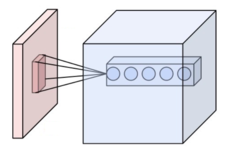
\includegraphics[width=0.65\columnwidth]{images/conv_layer.png} \caption{\href{https://en.wikipedia.org/wiki/File:Conv_layer.png}{Convolution Layers}}
\end{minipage}
\begin{minipage}{.3\textwidth}
  \centering
%  \textbf{Pooling Layers}\par\medskip
    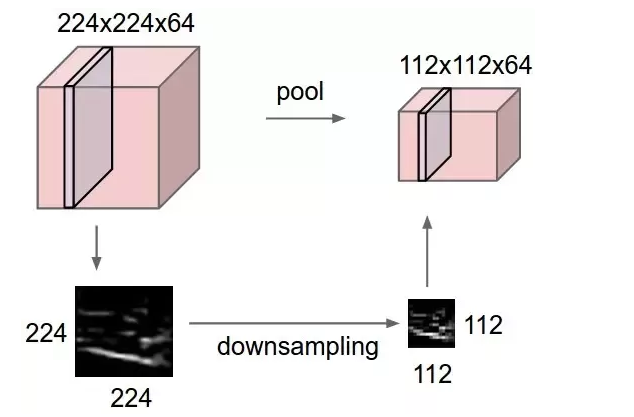
\includegraphics[width=0.65\columnwidth]{images/MaxpoolSample.png}
    \caption{\href{https://computersciencewiki.org/index.php/File:MaxpoolSample.png}{Pooling Layers}}
\end{minipage}
\begin{minipage}{.3\textwidth}
  \centering
%  \textbf{Fully-Connected Layers}\par\medskip
    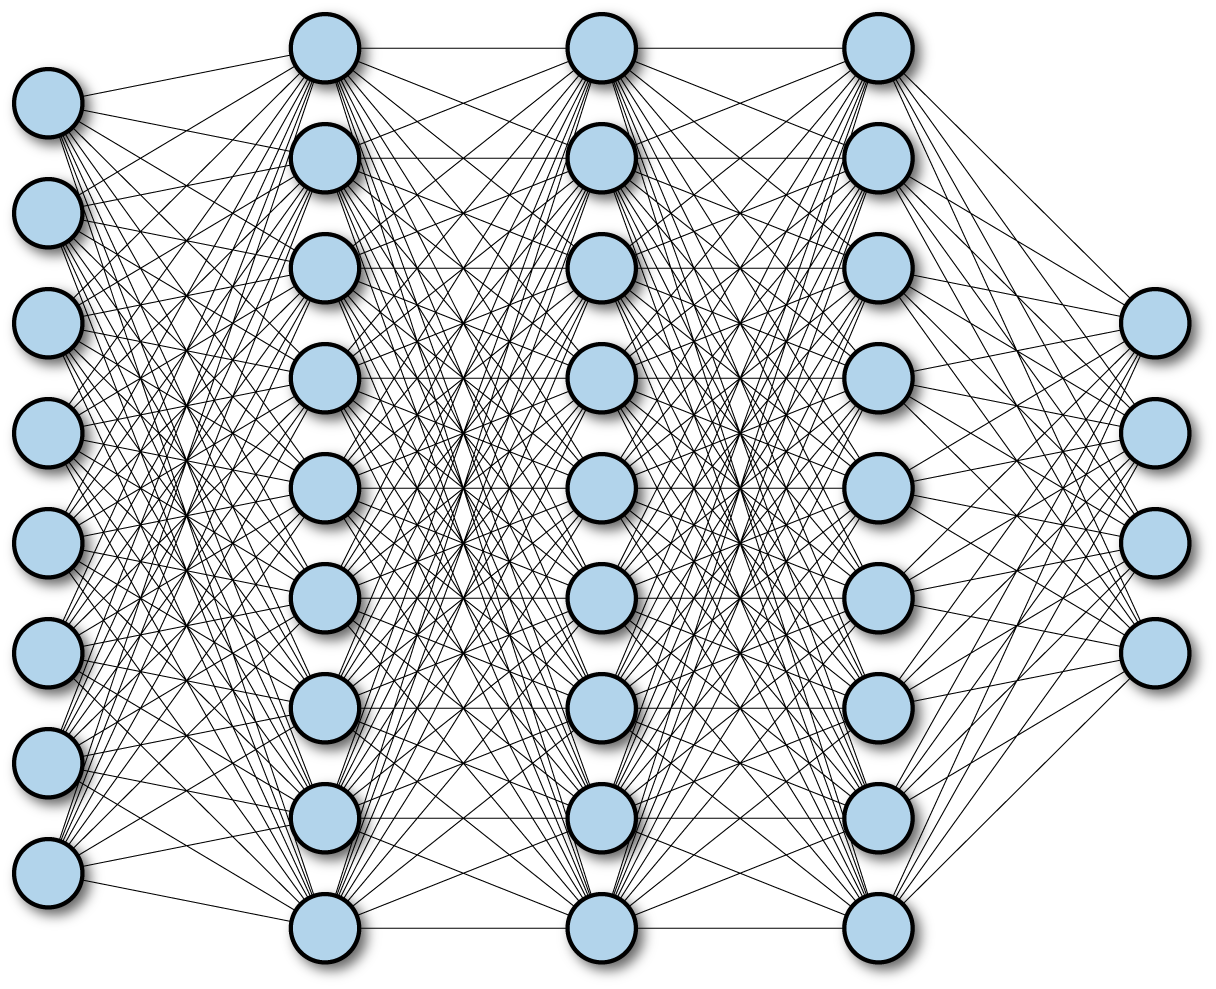
\includegraphics[width=0.55\columnwidth]{images/fully_connected.png}
    \caption{\href{https://www.oreilly.com/library/view/tensorflow-for-deep/9781491980446/ch04.html}{Dense Layers}}
\end{minipage}
\newline
\newline

\begin{minipage}{.4\textwidth}
  \centering
%  \textbf{Activation Functions}\par\medskip
    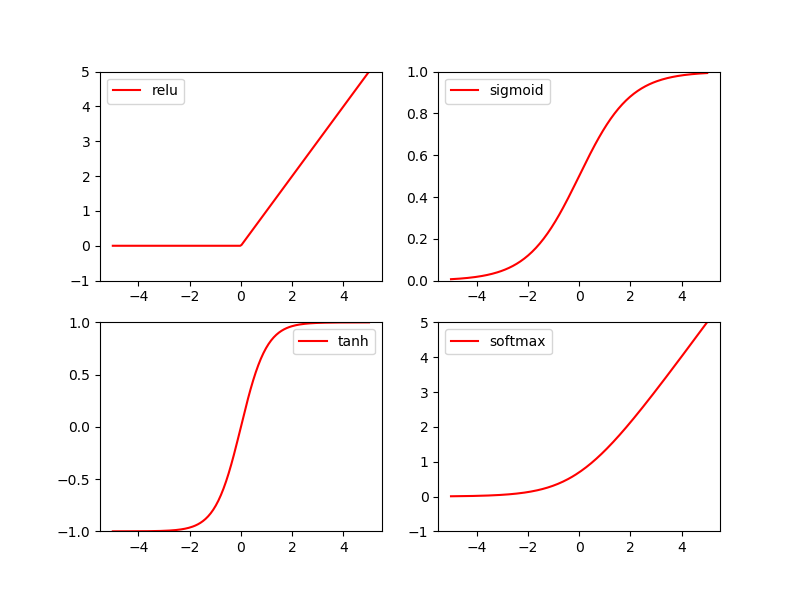
\includegraphics[width=0.65\columnwidth]{images/activation_function.png}
    \caption{\href{https://www.programmersought.com/article/12264689532/}{Activation Functions}}
\end{minipage}
\begin{minipage}{.5\textwidth}
  \centering
%  \textbf{Batch Normalization}\par\medskip
    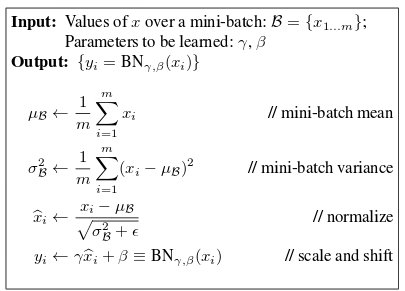
\includegraphics[width=0.65\columnwidth]{images/batch_normalization.png}
    \caption{\href{https://medium.com/@yagrawal.ya/batch-normalization-in-neural-networks-5c71e02eb45b}{Batch Normalization}}
\end{minipage}
\end{figure}


\pause 
\centering \Large{How should we put them together?}	

}

%%%%%%%%%%%%%%%%%%%%%%%%%%%%%%%%%%%%%%%%%%%%%%%%%%%%%%%%%%%%%%%%%%%%%%%%%%%%%%%%%%%%%%%%%%%%%%%


\frame{\frametitle{LeNet}
\begin{figure}
    \centering
    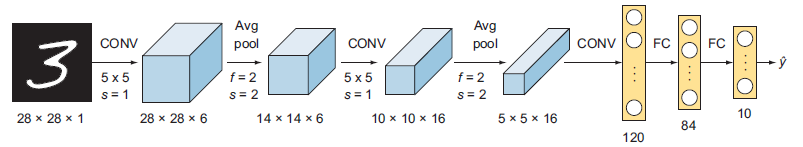
\includegraphics[width=1\columnwidth]{images/lenet-5_forward.png} \caption{\cite{elgendy2020vision}}
\end{figure}

\begin{itemize}
\item Conv filters were 5x5 , applied at stride 1
\item Subsampling (Pooling) layers were 2x2 applied at stride 2
\end{itemize}

}


\section{AlexNet}


\frame{\frametitle{AlexNet}
\begin{figure}
    \centering
    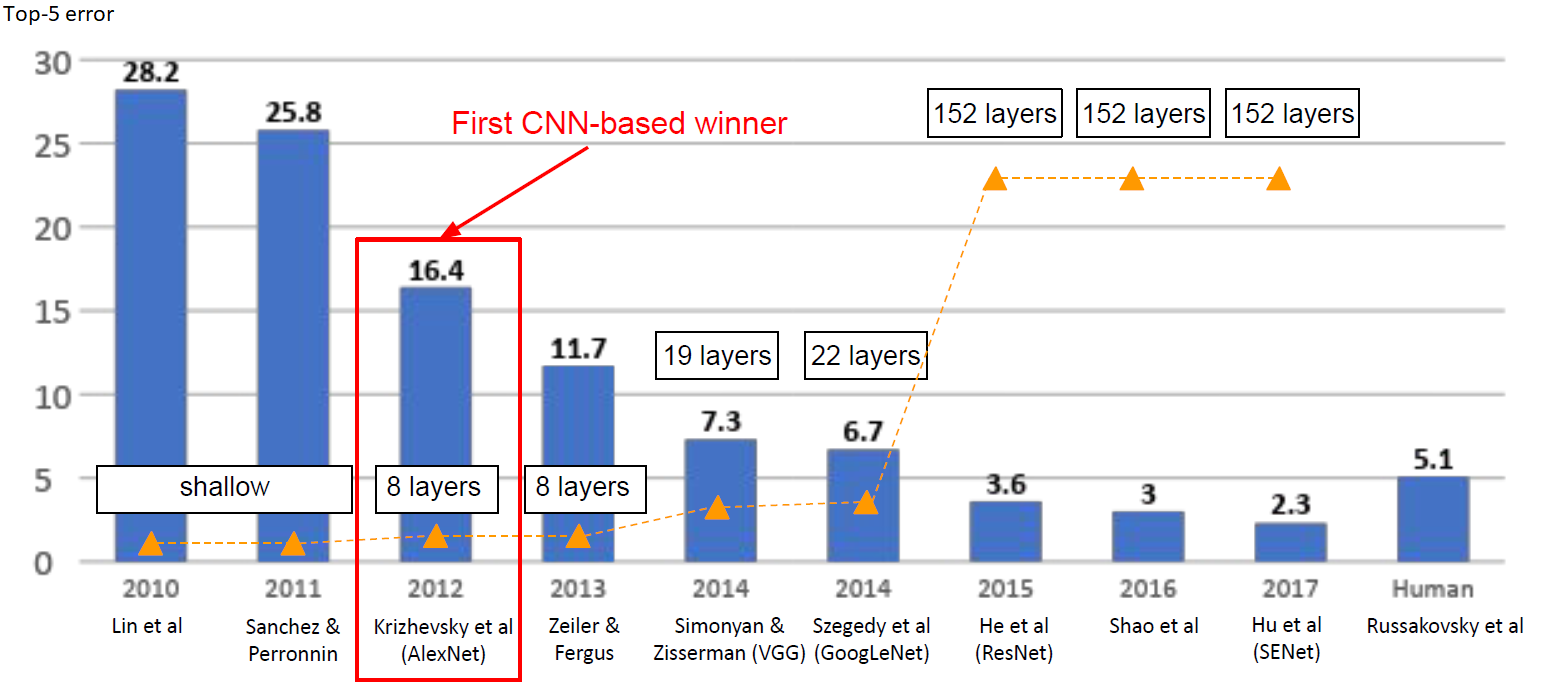
\includegraphics[width=1\columnwidth]{images/alexnet_imagenet.png} \caption{ImageNet Large Scale Visual Recognition Challenge (ILSVRC) winners}
\end{figure}}


\frame{\frametitle{AlexNet}
\begin{figure}
    \centering
    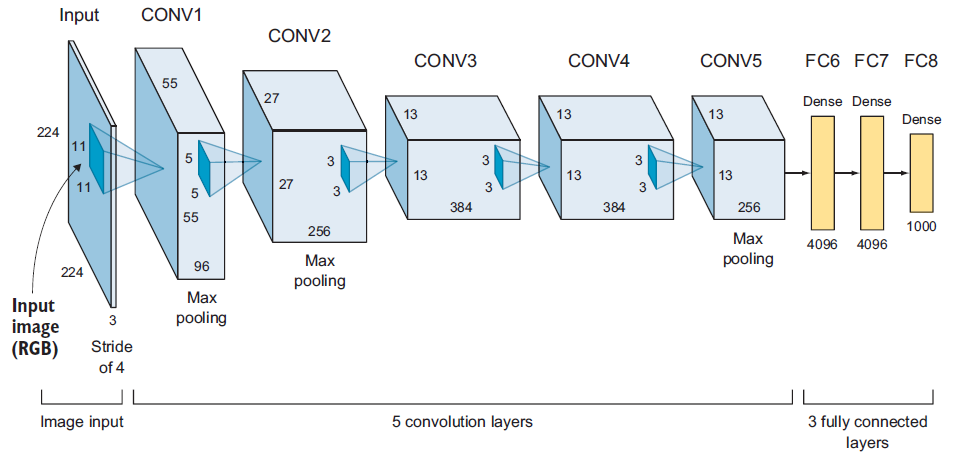
\includegraphics[width=0.9\columnwidth]{images/alexnet.png} \caption{\cite{elgendy2020vision}}
\end{figure}

\begin{itemize}
\item (CONV1): 96 11x11 filters applied at stride 4
\pause \item \color{red} Why is the output volume size 55?
\pause \item \color{blue} (227-11)/4+1 = 55
\end{itemize}

}

\frame{\frametitle{AlexNet}
\begin{figure}
    \centering
    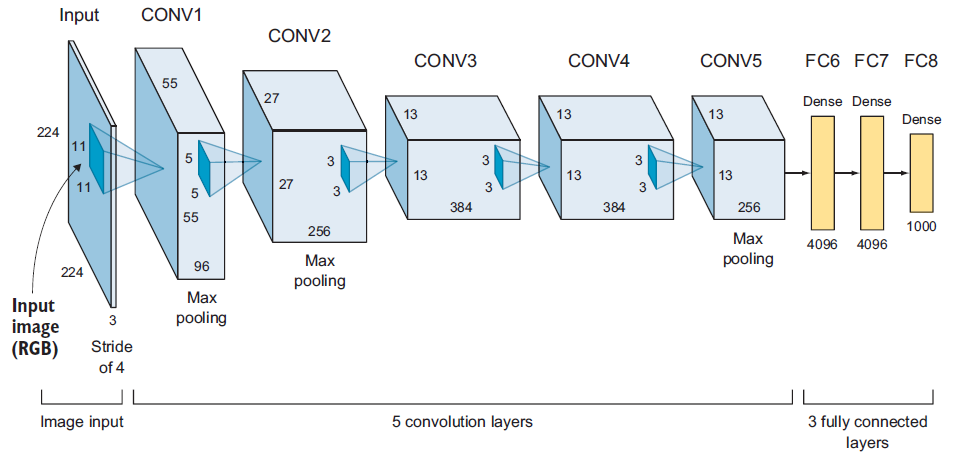
\includegraphics[width=0.9\columnwidth]{images/alexnet.png} \caption{\cite{elgendy2020vision}}
\end{figure}

\begin{itemize}
\item (CONV1): 96 11x11 filters applied at stride 4
\item \color{red} What is the total number of parameters in the first layer?
\pause \item \color{blue} (11*11*3 + 1)*96 = 35K
\end{itemize}

}


\frame{\frametitle{AlexNet}
\begin{figure}
    \centering
    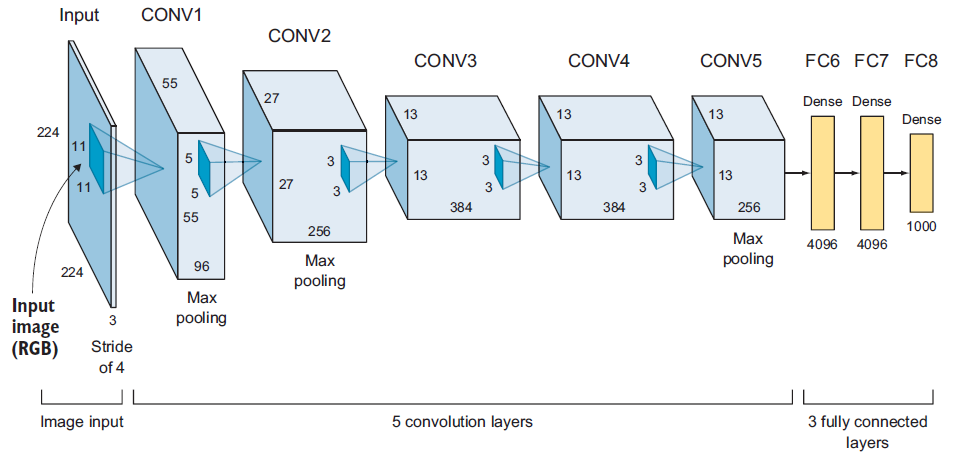
\includegraphics[width=0.9\columnwidth]{images/alexnet.png} \caption{\cite{elgendy2020vision}}
\end{figure}

\begin{itemize}
\item (POOL1): $3 \times 3$ filters applied at stride 2
\pause \item \color{red} Why is the output volume size 27?
\pause \item \color{blue} (55-3)/2+1 = 27
\end{itemize}

}


\frame{\frametitle{AlexNet}
\begin{figure}
    \centering
    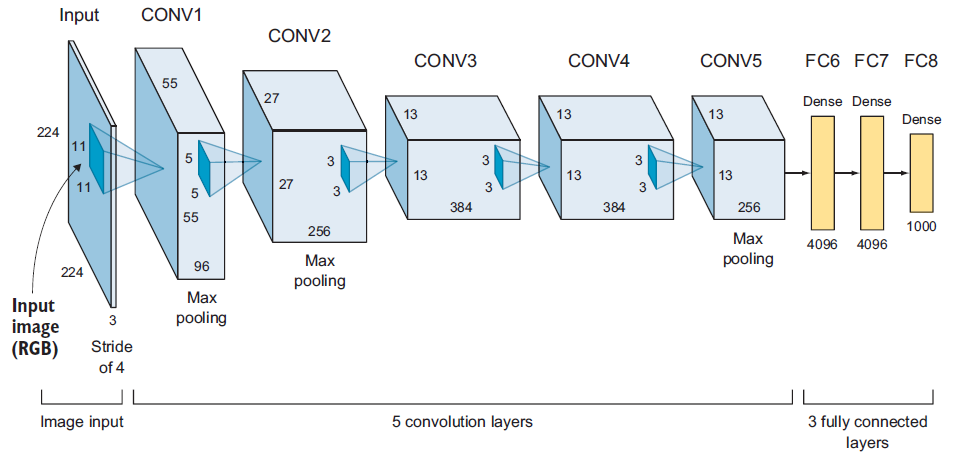
\includegraphics[width=0.9\columnwidth]{images/alexnet.png} \caption{\cite{elgendy2020vision}}
\end{figure}

\begin{itemize}
\item (POOL1): $3 \times 3$ filters applied at stride 2
\item \color{red} What is the number of parameters?
\pause \item \color{blue} Zero!
\end{itemize}

}

\frame{\frametitle{How is AlexNet Different from LeNet?}

\begin{columns}
\begin{column}{0.5\textwidth}
  \begin{itemize}
\item 62M parameters vs 61K parameters
\item ReLU vs Sigmoid (why?)
\item Use of Regularization Techniques (Dropout, Weight Decay) (why?)
\item Use of Normalization (why?)
\end{itemize}
\end{column}
\begin{column}{0.5\textwidth}  %%<--- here
   \begin{figure}
    \centering
    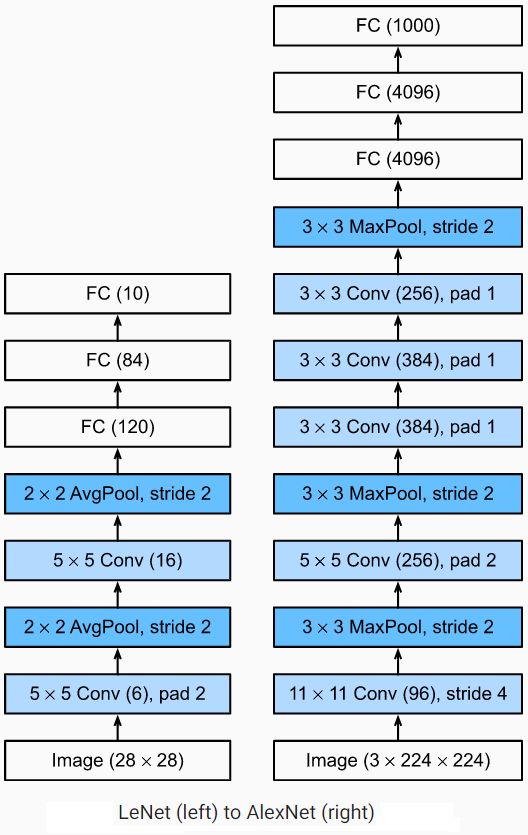
\includegraphics[width=0.7\columnwidth]{images/lenet_vs_alexnet.png} \caption{\cite{zhang2021dive}}
\end{figure}
\end{column}
\end{columns}

}



\section{VGGNet}


\frame{\frametitle{VGGNet}
\begin{figure}
    \centering
    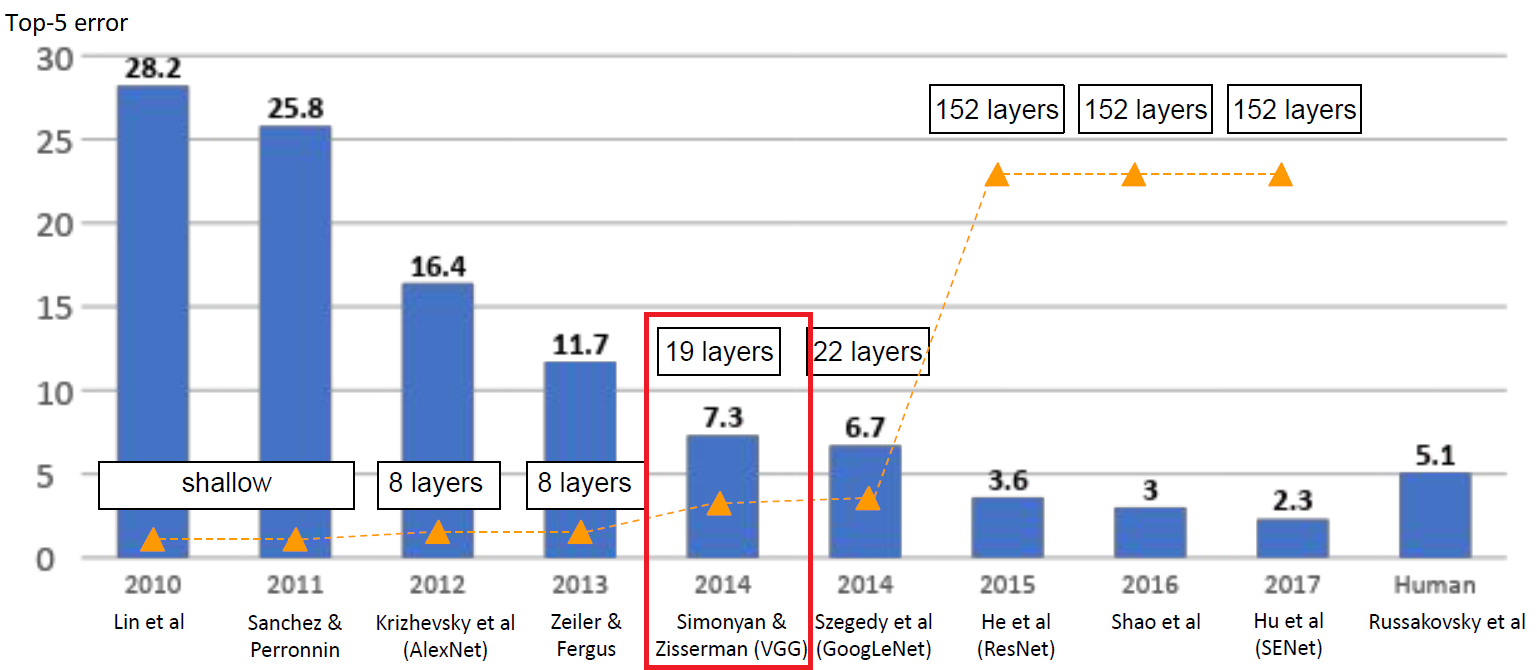
\includegraphics[width=1\columnwidth]{images/vgg_imagenet.png} \caption{ImageNet Large Scale Visual Recognition Challenge (ILSVRC) winners}
\end{figure}

}



\frame{\frametitle{VGGNet}
\begin{columns}
\begin{column}{0.5\textwidth}

\large{Do you see any difference?}

\onslide<2->{ \begin{itemize}
\item Smaller filters
\item  Deeper networks
\item Only $3 \times 3$ CONV with stride 1, pad 1 and $2 \times 2$ MAX POOL with stride 2
\end{itemize}}
\end{column}
\begin{column}{0.5\textwidth}  %%<--- here
   \begin{figure}
    \centering
    \onslide<1-> 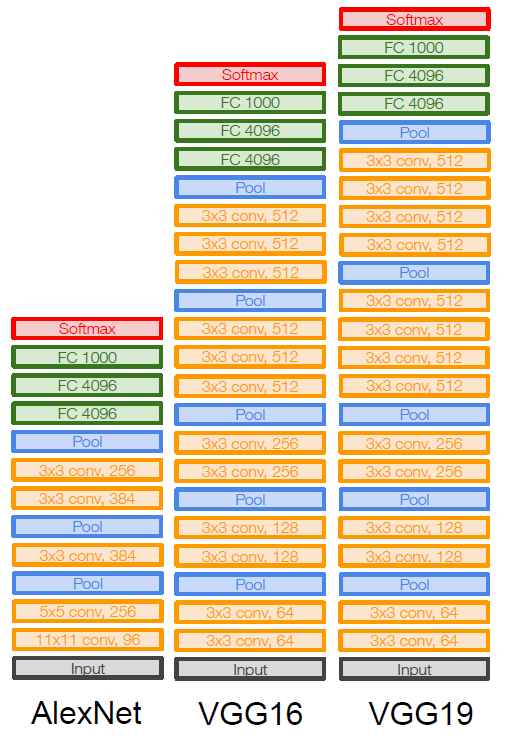
\includegraphics[width=0.8\columnwidth]{images/vgg.png}  \caption{\cite{wu2022cnn}}
\end{figure}
\end{column}
\end{columns}

}


\frame{\frametitle{VGGNet}
\begin{columns}
\begin{column}{0.6\textwidth}

\large{Why use smaller filters? ($3 \times 3$ conv)}

\begin{itemize}
\item \onslide<2-> Stack of three $3 \times 3$ conv (stride 1) layers
has same effective receptive field as
one $7 \times 7$ conv layer
\end{itemize}
\end{column}
\begin{column}{0.4\textwidth}  %%<--- here
   \begin{figure}
    \centering
    \onslide<1-> 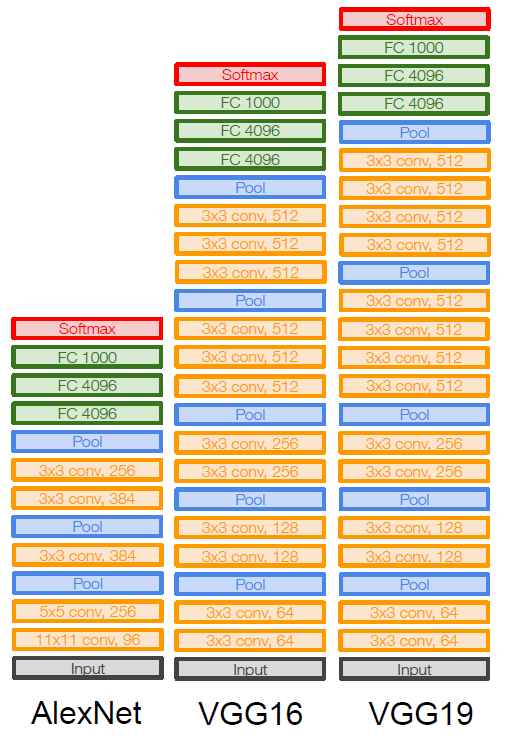
\includegraphics[width=0.8\columnwidth]{images/vgg.png} 
    \caption{\cite{wu2022cnn}}
\end{figure}
\end{column}
\end{columns}

}

\frame{\frametitle{VGGNet}

\Large{What is the effective receptive field of
three $3 \times 3$ conv (stride 1) layers?}

\begin{figure}
    \centering
    \only<1>{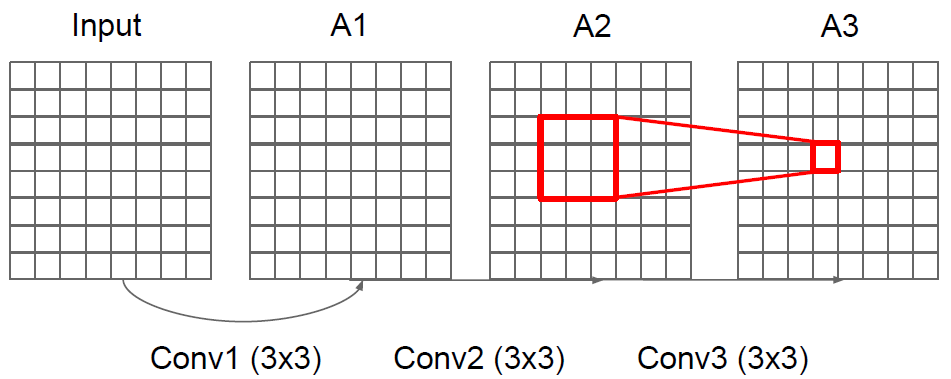
\includegraphics[width=1\columnwidth]{images/receptive1.png}}
    \only<2>{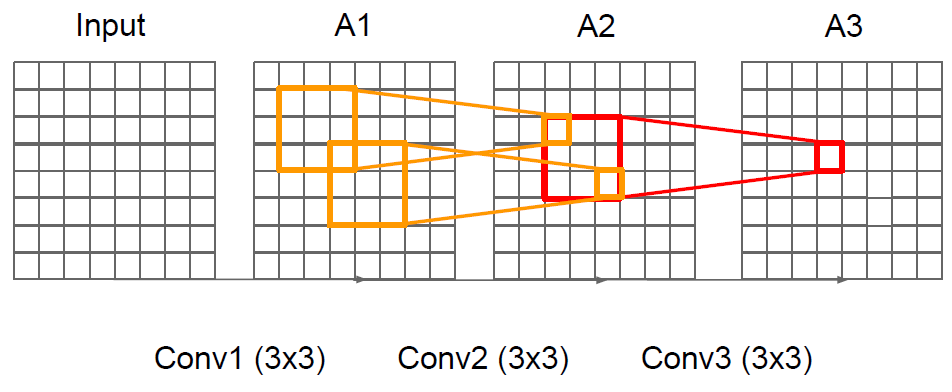
\includegraphics[width=1\columnwidth]{images/receptive2.png}}
    \only<3>{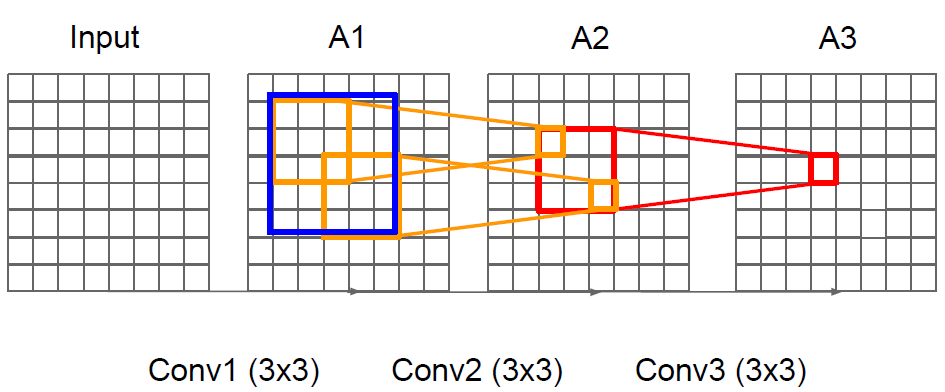
\includegraphics[width=1\columnwidth]{images/receptive3.png}}
    \only<4>{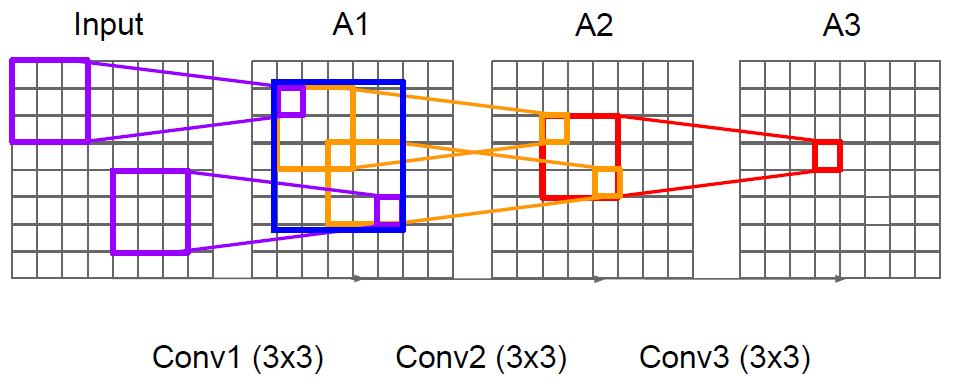
\includegraphics[width=1\columnwidth]{images/receptive4.png}}
    \only<5>{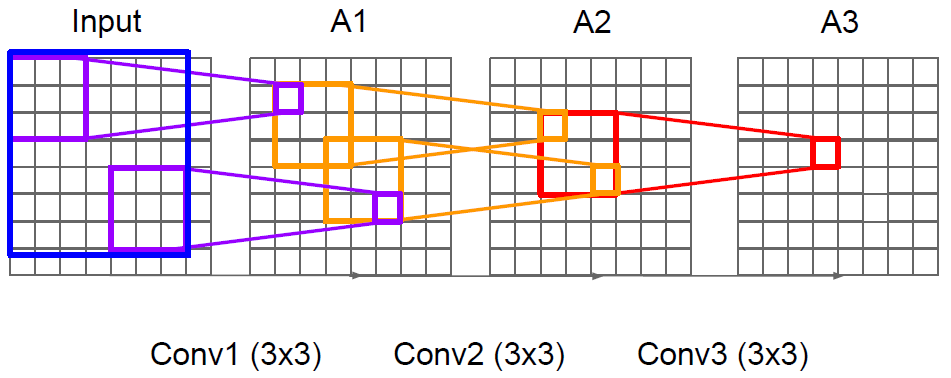
\includegraphics[width=1\columnwidth]{images/receptive5.png}} 
    \caption{\cite{wu2022cnn}}
\end{figure}

}


\frame{\frametitle{VGGNet}
\begin{columns}
\begin{column}{0.6\textwidth}

\large{Why use smaller filters? ($3 \times 3$ conv)}

\begin{itemize}
\item Stack of three $3 \times 3$ conv (stride 1) layers
has same effective receptive field as
one $7 \times 7$ conv layer

\item \onslide<2-> Deeper network means more non-linearities which leads to more capacity

\item \onslide<3-> Fewer parameters: $3 \times (3^2 C^2)$ vs.
$7^2 C^2$ for C channels per layer

\end{itemize}
\end{column}
\begin{column}{0.4\textwidth}  %%<--- here
   \begin{figure}
    \centering
    \onslide<1-> 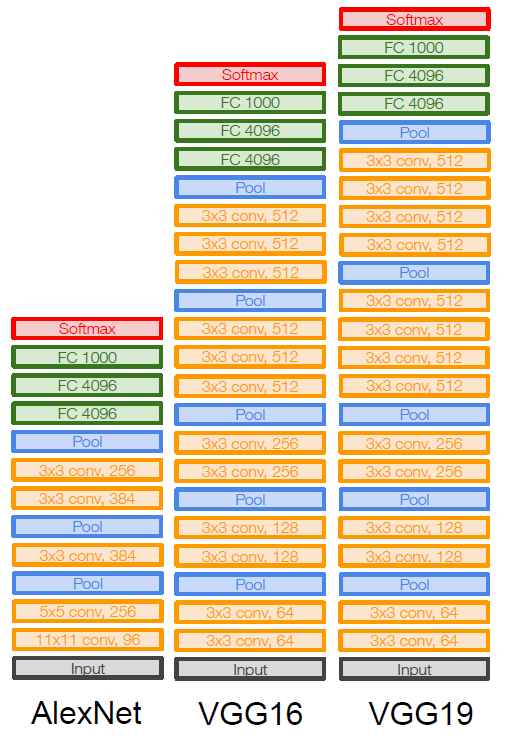
\includegraphics[width=0.8\columnwidth]{images/vgg.png} 
    \caption{\cite{wu2022cnn}}
\end{figure}
\end{column}
\end{columns}

}

\section{NiN}


\frame{\frametitle{Network in Network}
\begin{columns}
\begin{column}{0.4\textwidth}

\large{Do you see any difference?}

\onslide<2->{ \begin{itemize}
\item $1 \times 1$ Convolution
\item  Global Average Pooling(GAP) layer instead of FC layers
\end{itemize}}
\end{column}
\begin{column}{0.6\textwidth}  %%<--- here
   \begin{figure}
    \centering
    \onslide<1-> 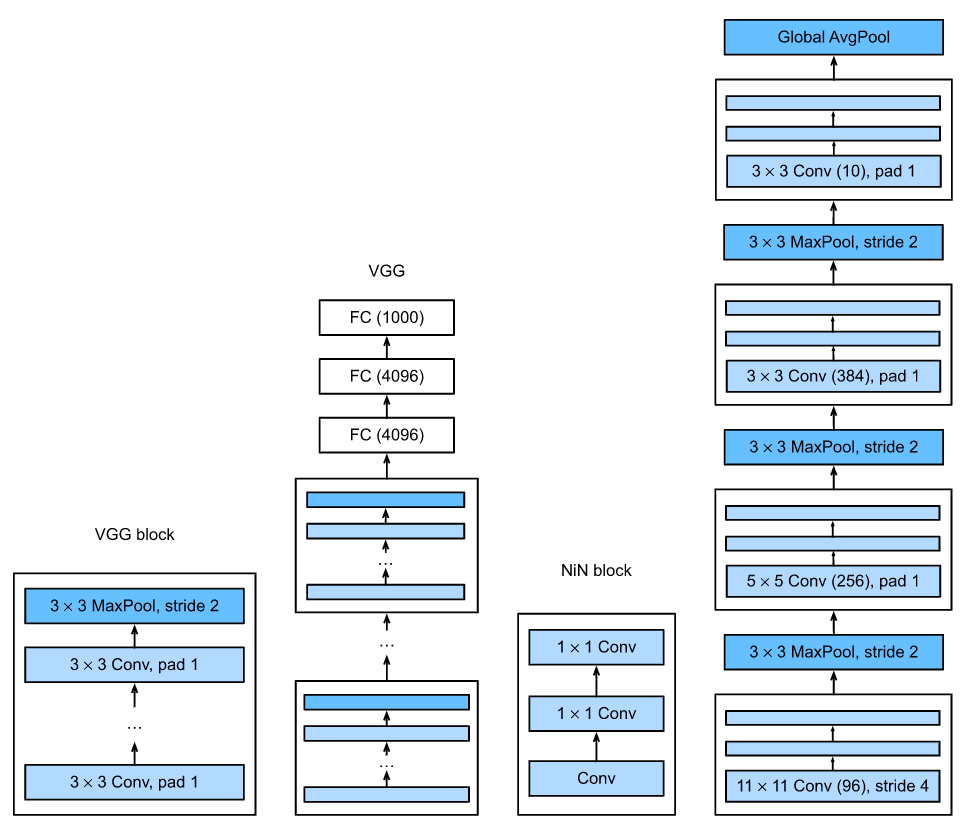
\includegraphics[width=0.9\columnwidth]{images/VGG_vs_NiN.png} \caption{\cite{zhang2021dive}}
\end{figure}
\end{column}
\end{columns}

}


\frame{\frametitle{$1 \times 1$ Convolution}

\begin{figure}
    \centering
    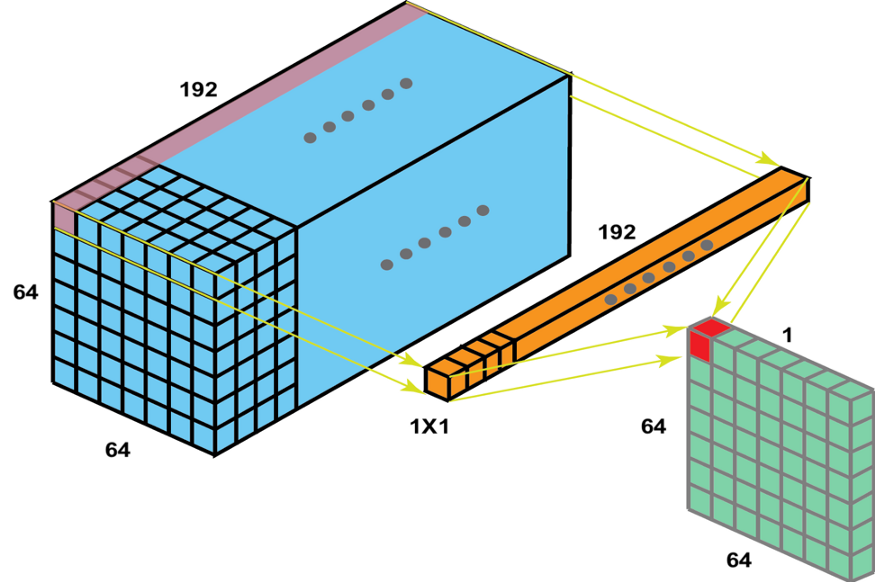
\includegraphics[width=0.8\columnwidth]{images/1by1conv.png}
 \caption{\href{https://miro.medium.com/max/875/1*dNaikOfrGzUaJ2EzRIl4tw.png}{ $1 \times 1$ Convolution}}
\end{figure}

}

\frame{\frametitle{$1 \times 1$ Conv Use Case}

\begin{itemize}
\item Assume we want to transform a $32 \times 32 \times 200$ tensor to a $32 \times 32 \times 32$ one using 32 $5 \times 5$ filters. Thus, we need $(32 \times 32 \times 200) \times (5 \times 5 \times 32) \approx 163M$ operations!
\pause  \item Instead we can use $1 \times 1$ convolution:

\begin{figure}
    \centering
    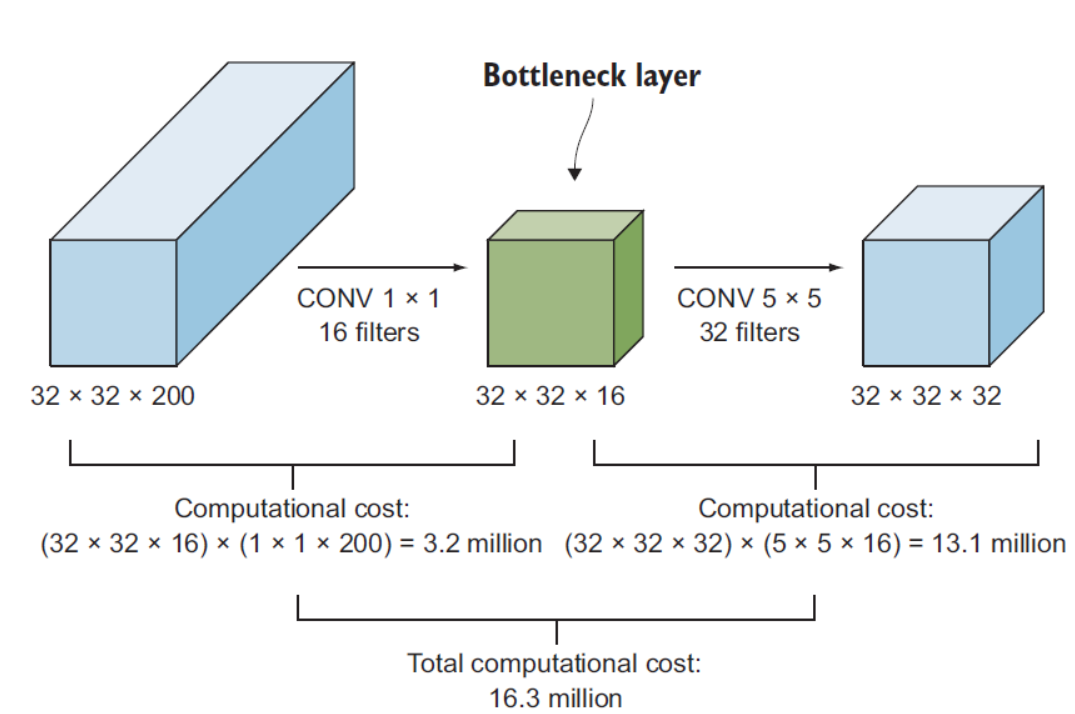
\includegraphics[width=0.7\columnwidth]{images/1by1conv_computation.png}
\caption{\cite{elgendy2020vision}}
\end{figure}

\end{itemize}

}


\frame{\frametitle{Global Average Pooling}

Similar to max pooling layers, GAP layers are used to reduce the spatial dimensions of a three-dimensional tensor. However, GAP layers perform a more extreme type of dimensionality reduction, where a tensor with dimensions $h \times w \times d$ is reduced in size to have dimensions $1 \times 1 \times d$. GAP layers reduce each $h \times w$ feature map to a single number by simply taking the average of all hw values.

\begin{figure}
    \centering
    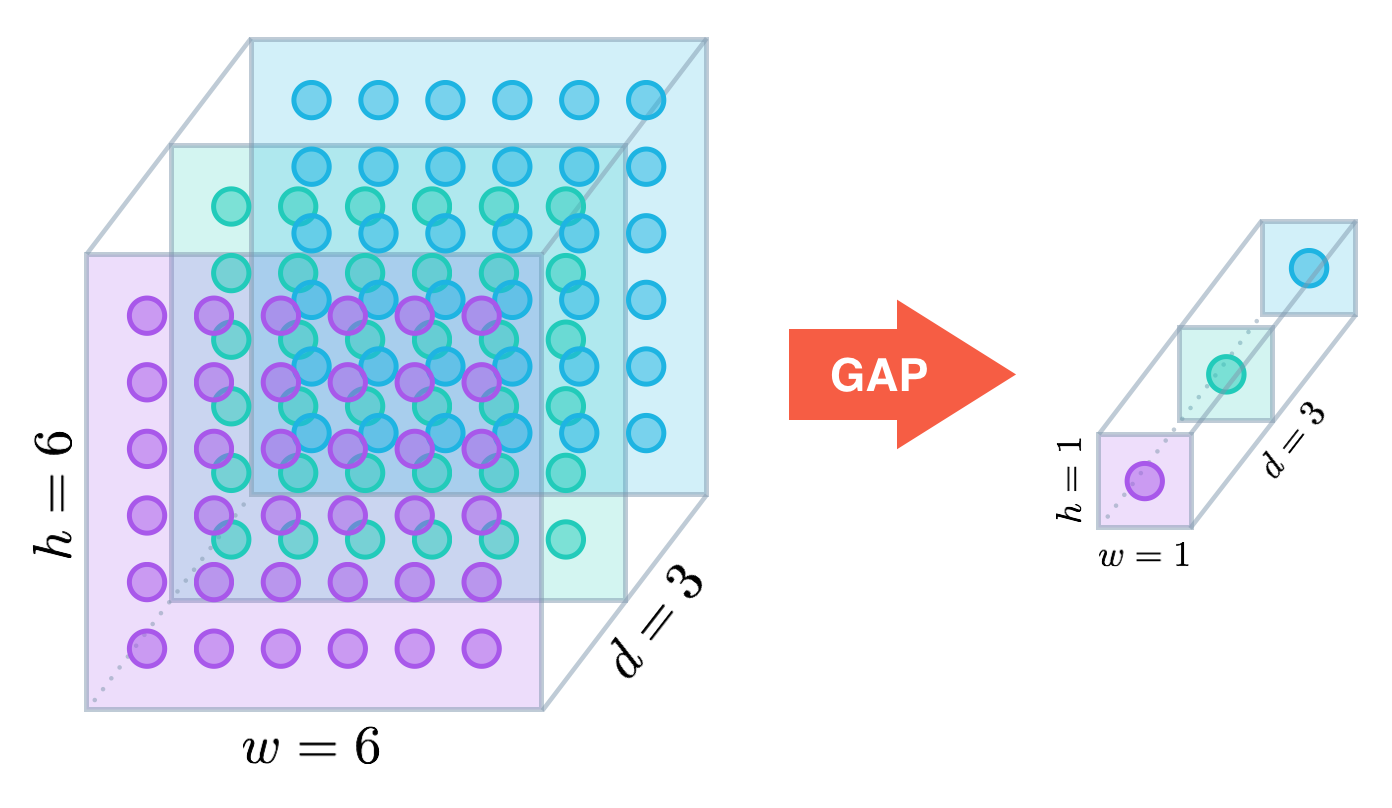
\includegraphics[width=0.6\columnwidth]{images/global_average_pooling.png}
 \caption{\href{https://alexisbcook.github.io/2017/global-average-pooling-layers-for-object-localization/}{ GAP}}
\end{figure}

}


\frame{\frametitle{Why GAP?}

\begin{itemize}
\item GAP is used to replace the traditional fully connected layers in CNN.
\item There is no parameter to optimize in the GAP
thus overfitting is avoided at this layer
\item GAP sums out the spatial information, thus it is more robust to spatial translations of the input.
\end{itemize}

\begin{figure}
    \centering
    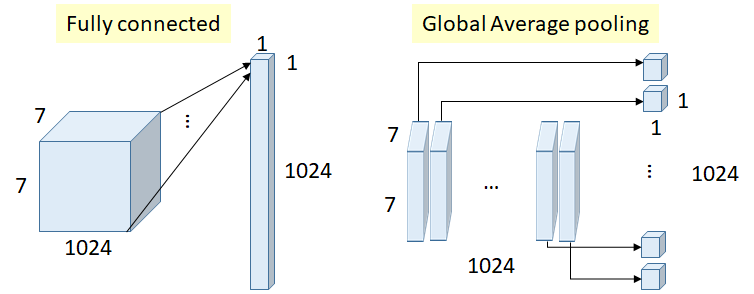
\includegraphics[width=0.8\columnwidth]{images/FC_vs_GAP.png}
 \caption{\href{https://towardsdatascience.com/review-nin-network-in-network-image-classification-69e271e499ee}{ FC Layer vs GAP Layer}}
\end{figure}

}


\section{GoogLeNet}


\frame{\frametitle{GoogLeNet}

\begin{figure}
    \centering
    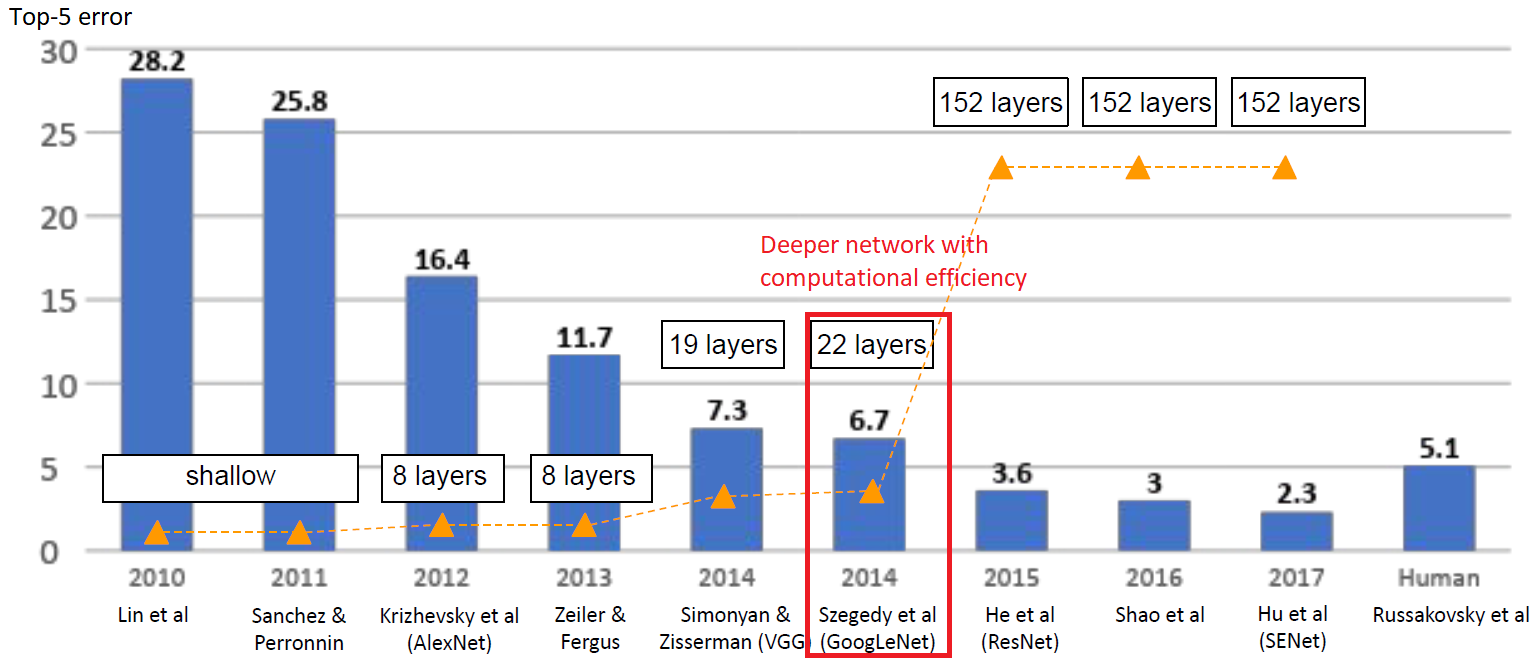
\includegraphics[width=1\columnwidth]{images/googlenet_imagenet.png} \caption{ImageNet Large Scale Visual Recognition Challenge (ILSVRC) winners}
\end{figure}
}


\frame{\frametitle{GoogLeNet}

\begin{columns}
\begin{column}{0.5\textwidth}
  \begin{itemize}
\item Only 5 million parameters! (12x less than AlexNet and 27x less than VGG-16)
\item Efficient “Inception” module
\item No longer multiple expensive FC layers
\end{itemize}
\end{column}
\begin{column}{0.5\textwidth}  %%<--- here
   \begin{figure}
    \centering
    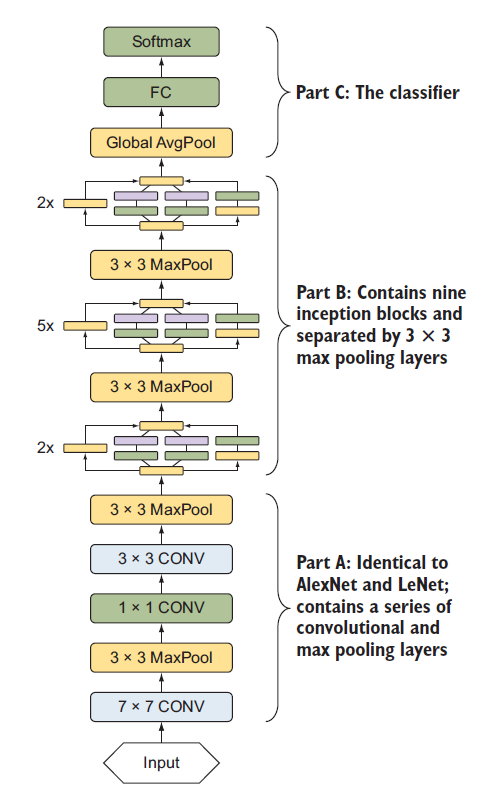
\includegraphics[width=0.7\columnwidth]{images/googlenet_complete.png} \caption{\cite{elgendy2020vision}}
\end{figure}
\end{column}
\end{columns}
}


\frame{\frametitle{GoogLeNet}

Inception modules instead of classical CNNs for feature extraction

\begin{figure}
    \centering
    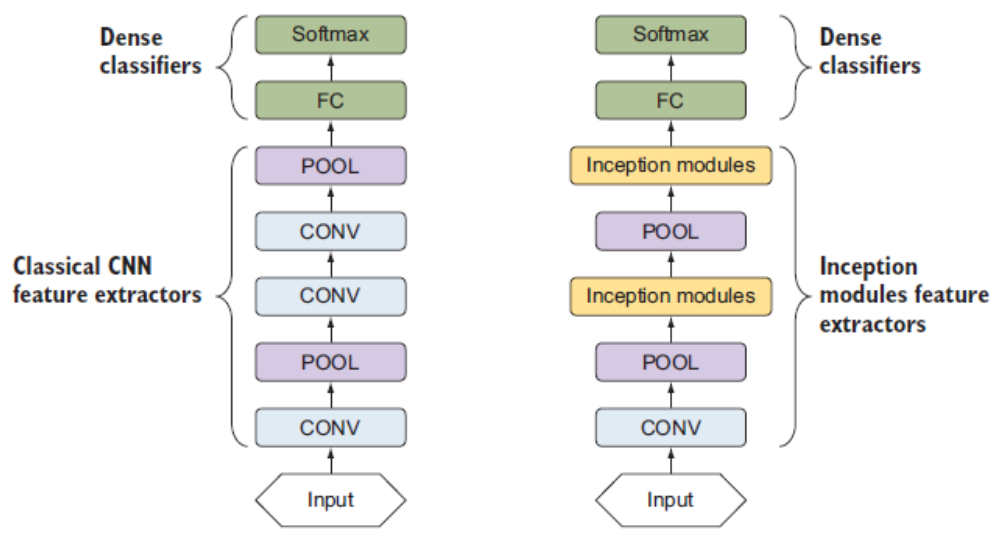
\includegraphics[width=0.9\columnwidth]{images/classical_cnn_vs_inception_module.png}
    \caption{\cite{elgendy2020vision}}
\end{figure}
}


\frame{\frametitle{Naive Inception Module}

\begin{itemize}
\item Apply parallel filter operations on the input from previous layer
\item Multiple receptive field sizes for convolution ($1 \times 1$, $3 \times 3$, $5 \times 5$)
\item Pooling operation ($3 \times 3$)
\item Concatenate all filter outputs together channel-wise
\end{itemize}

\begin{figure}
    \centering
    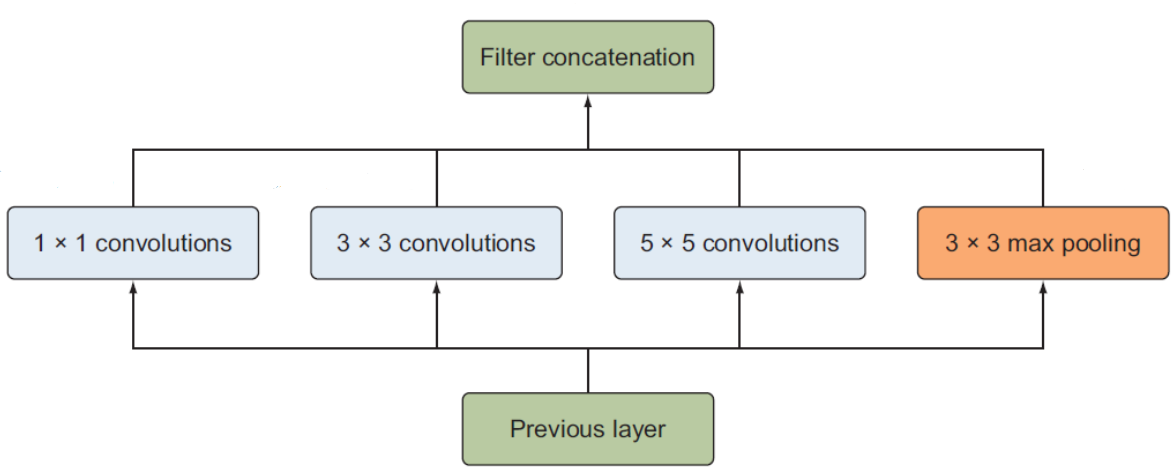
\includegraphics[width=0.9\columnwidth]{images/naive_inception.png}
    \caption{\cite{elgendy2020vision}}
\end{figure}
}

\frame{\frametitle{Naive Inception Module}

\begin{itemize}
\only<1>{ \item What are the output sizes of all different filter operations?}
\only<2>{\item What are the output sizes of all different filter operations?}
\only<3>{\item What is output size after filter concatenation?}
\only<4>{\item What is output size after filter concatenation?}
\only<5>{\item What is the problem with this?}
\only<6>{\item What is the problem with this?
\item Computational complexity!
\begin{itemize}
		\item Conv Ops:
		\item $[1 \times 1 \; \text{conv}, 128] \; 28 \times 28 \times 128 \times 1 \times 1 \times 256$
		\item $[3 \times 3 \; \text{conv}, 192] \; 28 \times 28 \times 192 \times 3 \times 3 \times 256$
		\item $[5 \times 5 \; \text{conv}, 96] \; \; \; 28 \times 28 \times 96 \times 5 \times 5 \times 256$
		\item Total:  854M  ops
\end{itemize}
\item Pooling layer preserves feature
depth, which means total depth after
concatenation can only grow at every
layer!
}
\end{itemize}

\begin{figure}
    \centering
    \only<1>{ 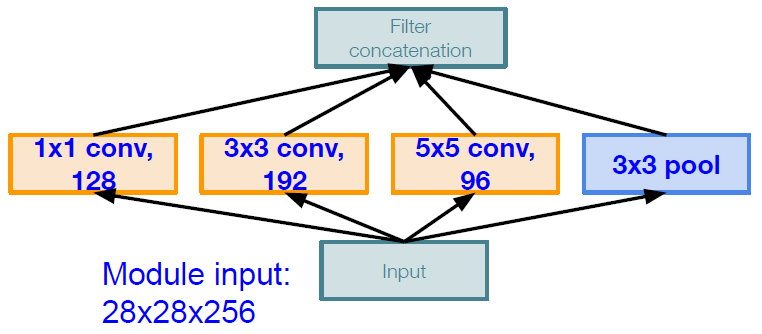
\includegraphics[width=0.9\columnwidth]{images/naive_inception_example1.png}}
        \only<2>{ 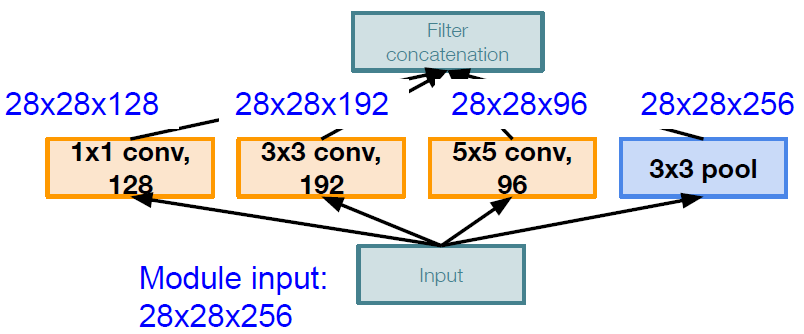
\includegraphics[width=0.9\columnwidth]{images/naive_inception_example2.png}}
	\only<3>{ 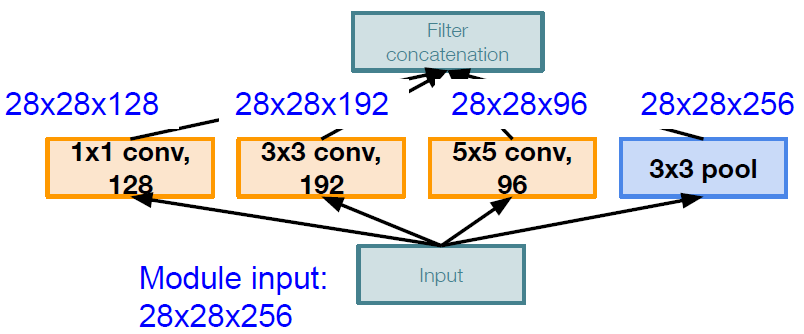
\includegraphics[width=0.9\columnwidth]{images/naive_inception_example2.png}}
        \only<4>{ 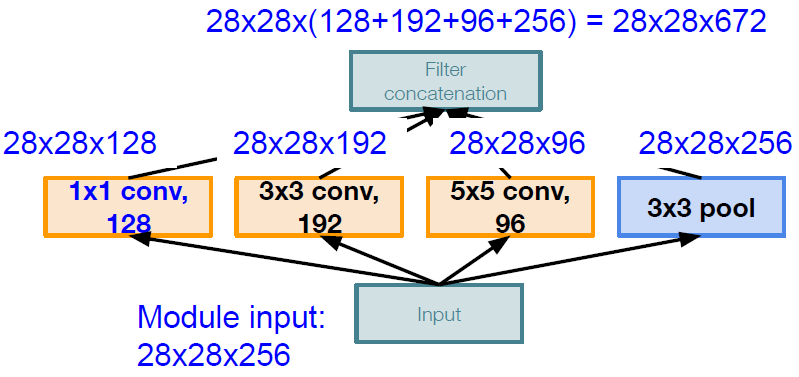
\includegraphics[width=0.9\columnwidth]{images/naive_inception_example3.png}}
        \only<5>{ 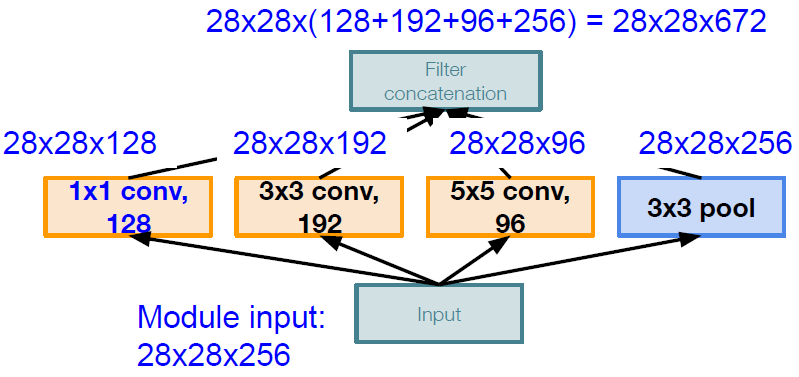
\includegraphics[width=0.9\columnwidth]{images/naive_inception_example3.png}}
        \only<6>{ 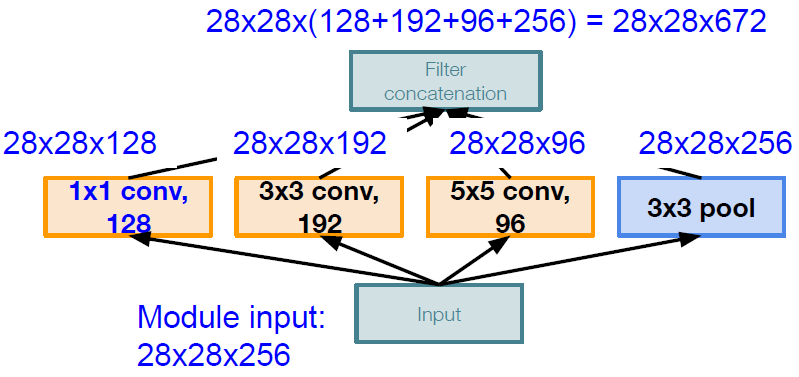
\includegraphics[width=0.6\columnwidth]{images/naive_inception_example3.png}}
\caption{\cite{wu2022cnn}}
\end{figure}
}


\frame{\frametitle{Inception Module}

\begin{itemize}
\item Any Solution?
\pause \item “bottleneck” layers that use $1 \times 1$ convolutions to reduce feature channel size
\end{itemize}

\begin{figure}
    \centering
     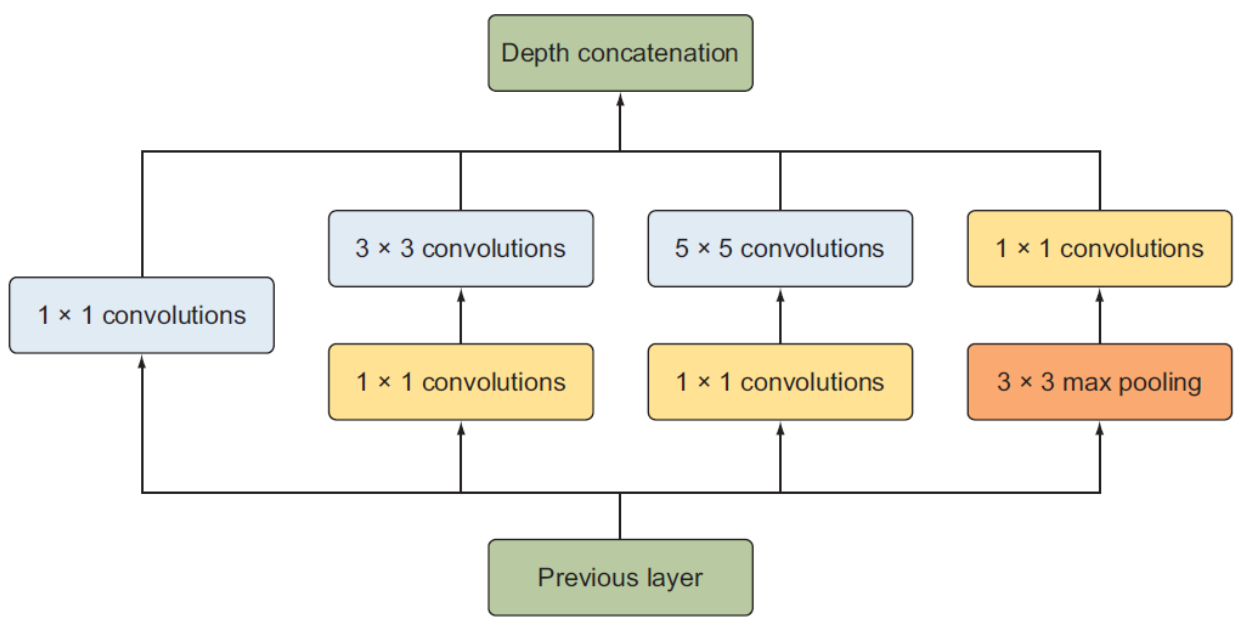
\includegraphics[width=0.9\columnwidth]{images/inception_module.png}
    \caption{\cite{elgendy2020vision}}
\end{figure}}

\frame{\frametitle{Dimension Reduction in Inception Module}

\begin{itemize}
\item Using same parallel layers as naive example, and adding “$1 \times 1$ conv, 64 filter” bottlenecks
\begin{itemize}
		\item $[1 \times 1 \; \text{conv}, 64] \; 28 \times 28 \times 64 \times 1 \times 1 \times 256$
		\item $[1 \times 1 \; \text{conv}, 64] \; 28 \times 28 \times 64 \times 1 \times 1 \times 256$
		\item $[1 \times 1 \; \text{conv}, 128] \; 28 \times 28 \times 128 \times 1 \times 1 \times 256$
		\item $[3 \times 3 \; \text{conv}, 192] \; 28 \times 28 \times 192 \times 3 \times 3 \times 64$
		\item $[5 \times 5 \; \text{conv}, 96] \; 28 \times 28 \times 96 \times 5 \times 5 \times 64$
		\item $[1 \times 1 \; \text{conv}, 64] \; 28 \times 28 \times 64 \times 1 \times 1 \times 256$
		\item Total:  358M  ops
\end{itemize}
\item Compared to 854M ops for naive version Bottleneck can also reduce depth after pooling layer
\end{itemize}

\begin{figure}
    \centering
     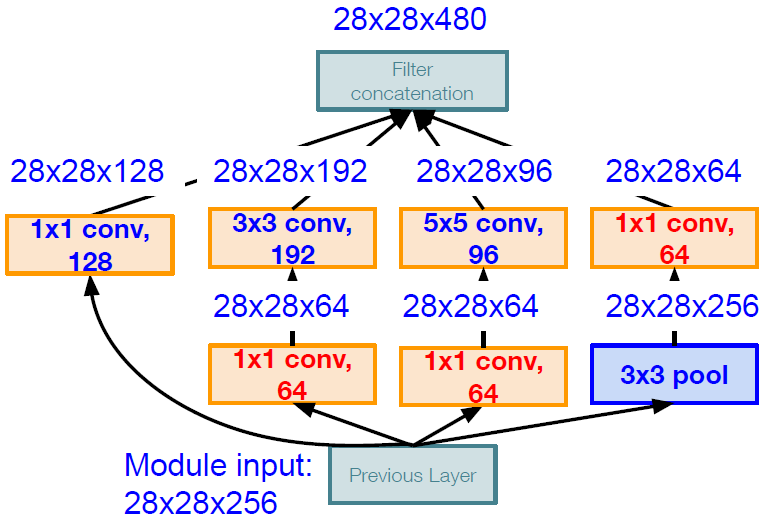
\includegraphics[width=0.35\columnwidth]{images/naive_inception_example4.png}
\caption{\cite{wu2022cnn}}
\end{figure}}

\section{ResNet}

\frame{\frametitle{ResNet}
\begin{figure}
    \centering
    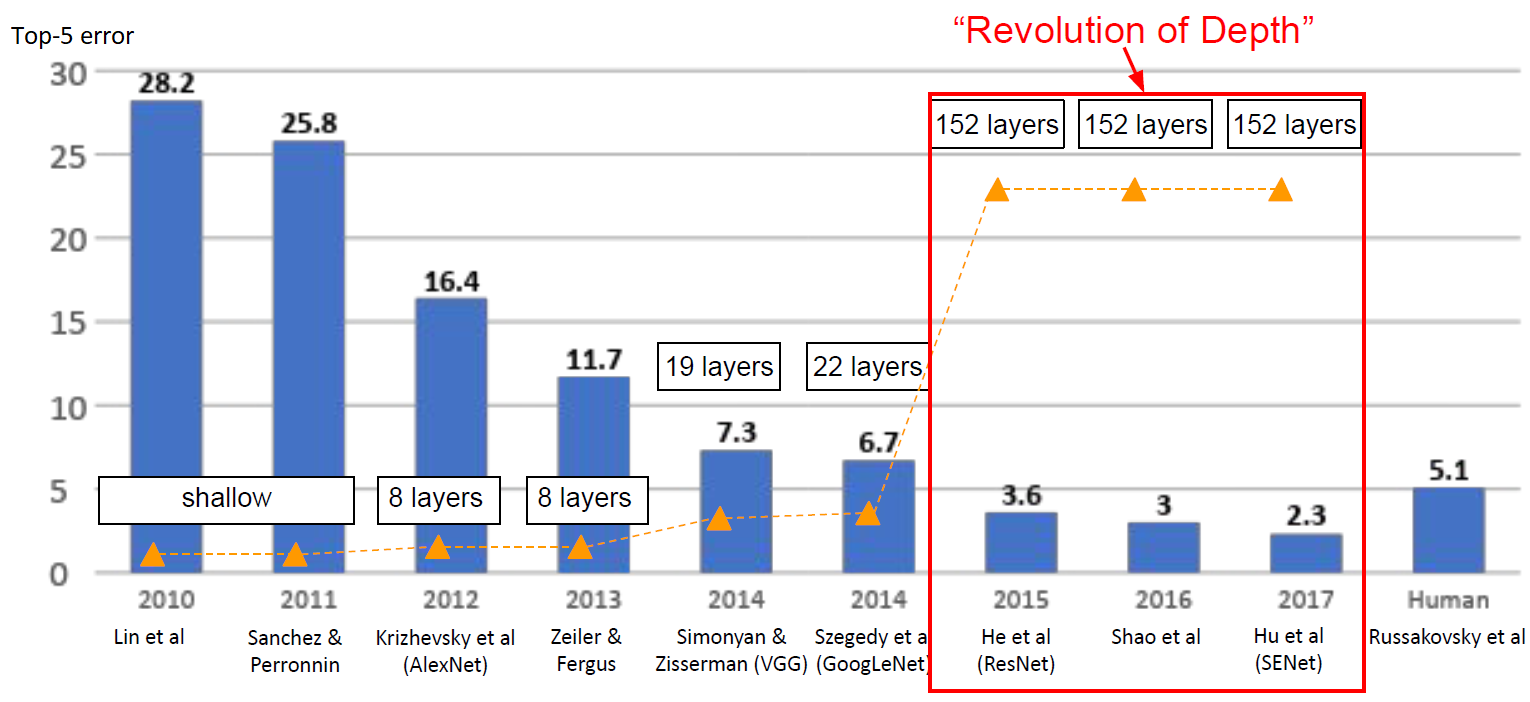
\includegraphics[width=1\columnwidth]{images/resnet_imagenet.png} \caption{ImageNet Large Scale Visual Recognition Challenge (ILSVRC) winners}
\end{figure}}


\frame{\frametitle{ResNet}

\begin{columns}
\begin{column}{0.7\textwidth}
  \begin{itemize}
\onslide<1-> \item A very deep network using residual connections
\onslide<1-> \item What happens when we continue stacking deeper layers on a “plain” convolutional
\onslide<2-> 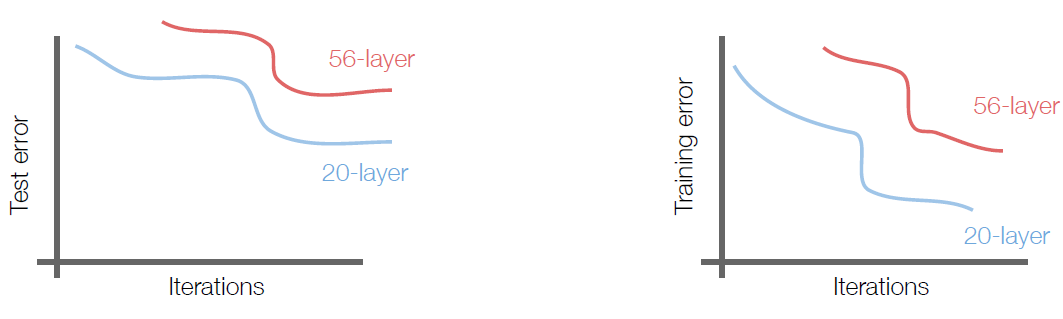
\includegraphics[width=0.9\columnwidth]{images/layers_error.png}
\onslide<3-> \item The deeper model performs worse, but it’s not caused by overfitting!
\end{itemize}
\end{column}
\begin{column}{0.3\textwidth}  %%<--- here
   \begin{figure}
    \centering
    \onslide<1-> 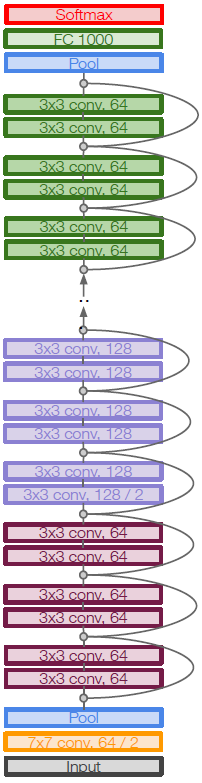
\includegraphics[width=0.5\columnwidth]{images/resnet.png} \caption{\cite{wu2022cnn}}
\end{figure}
\end{column}
\end{columns}
}

\frame{\frametitle{ResNet}

\begin{columns}
\begin{column}{0.7\textwidth}
  \begin{itemize}
\onslide<1-> \item Fact: Deep models have more representation power
(more parameters) than shallower models.
\onslide<1-> \item Hypothesis: the problem is an optimization problem,
deeper models are harder to optimize
\onslide<2-> \item What should the deeper model learn to be at least
as good as the shallower model?
\end{itemize}
\end{column}
\begin{column}{0.3\textwidth}  %%<--- here
   \begin{figure}
    \centering
    \onslide<1-> 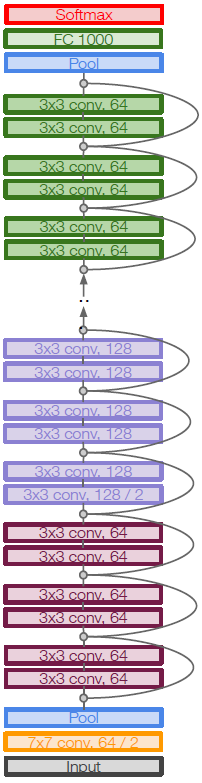
\includegraphics[width=0.5\columnwidth]{images/resnet.png} \caption{\cite{wu2022cnn}}
\end{figure}
\end{column}
\end{columns}
}

\frame{\frametitle{Skip Connection}

Use network layers to fit a residual mapping instead of directly trying to fit a
desired underlying mapping

\begin{figure}
    \centering
     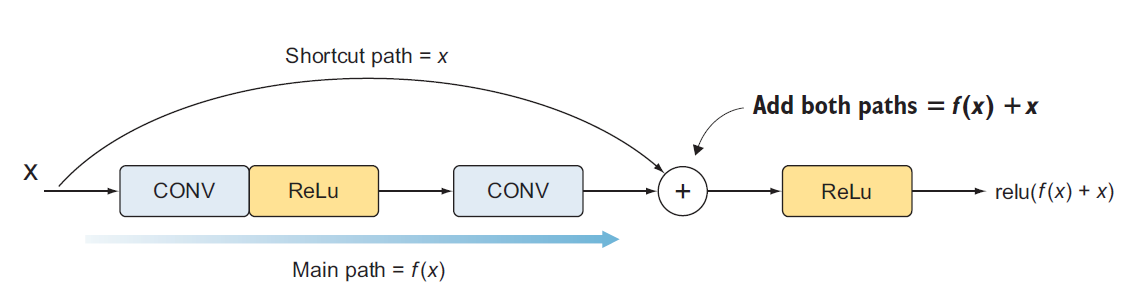
\includegraphics[width=0.9\columnwidth]{images/skip_connection.png}
    \caption{\cite{elgendy2020vision}}
\end{figure}}


\frame{\frametitle{Full ResNet Architecture}

\begin{columns}
\begin{column}{0.5\textwidth}
  \begin{itemize}
\item Stack residual blocks
\item Every residual block has two $3 \times 3$ conv layers
\item Periodically, double size of filters and downsample spatially using stride 2 (/2 in each dimension)
\item Additional conv layer at the beginning (stem)
\item No FC layers besides FC 1000 to output classes
\item Global average pooling layer after last conv layer
\item Batch Normalization after every CONV layer
\item No dropout used
\end{itemize}
\end{column}
\begin{column}{0.5\textwidth}  %%<--- here
   \begin{figure}
    \centering
    \onslide<1-> 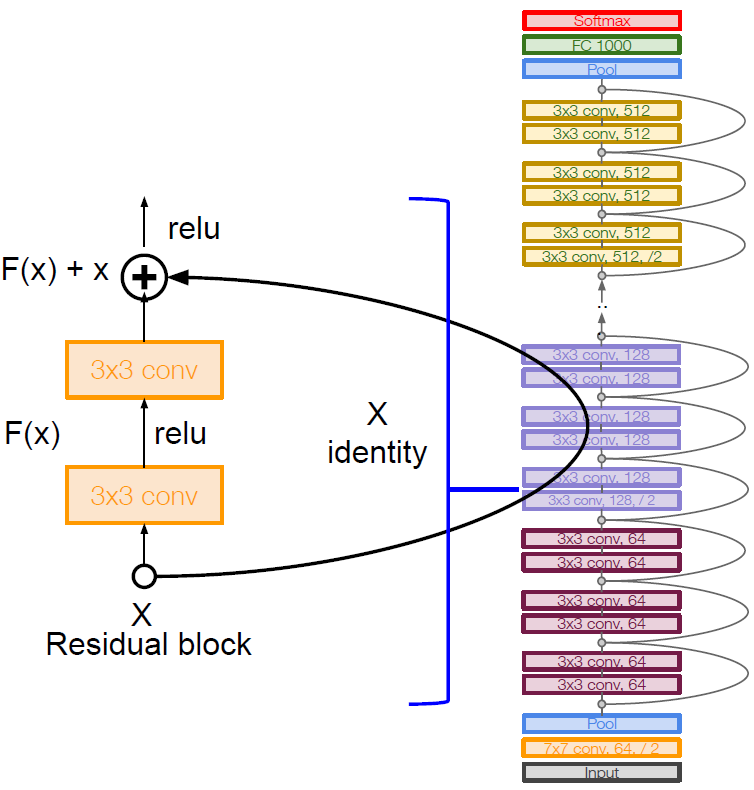
\includegraphics[width=1\columnwidth]{images/resent_with_skipconnection.png} \caption{\cite{wu2022cnn}}
\end{figure}
\end{column}
\end{columns}
}

\section{ResNeXt}

\frame{\frametitle{ResNeXt}

\begin{itemize}
\item Increases width of residual block through multiple parallel pathways (similar to Inception module)
\item Using g pathways for computational efficiency (why?)
\item What is the purpose of the last $1 \times 1$ CONV layer?
\end{itemize}

\begin{figure}
    \centering
     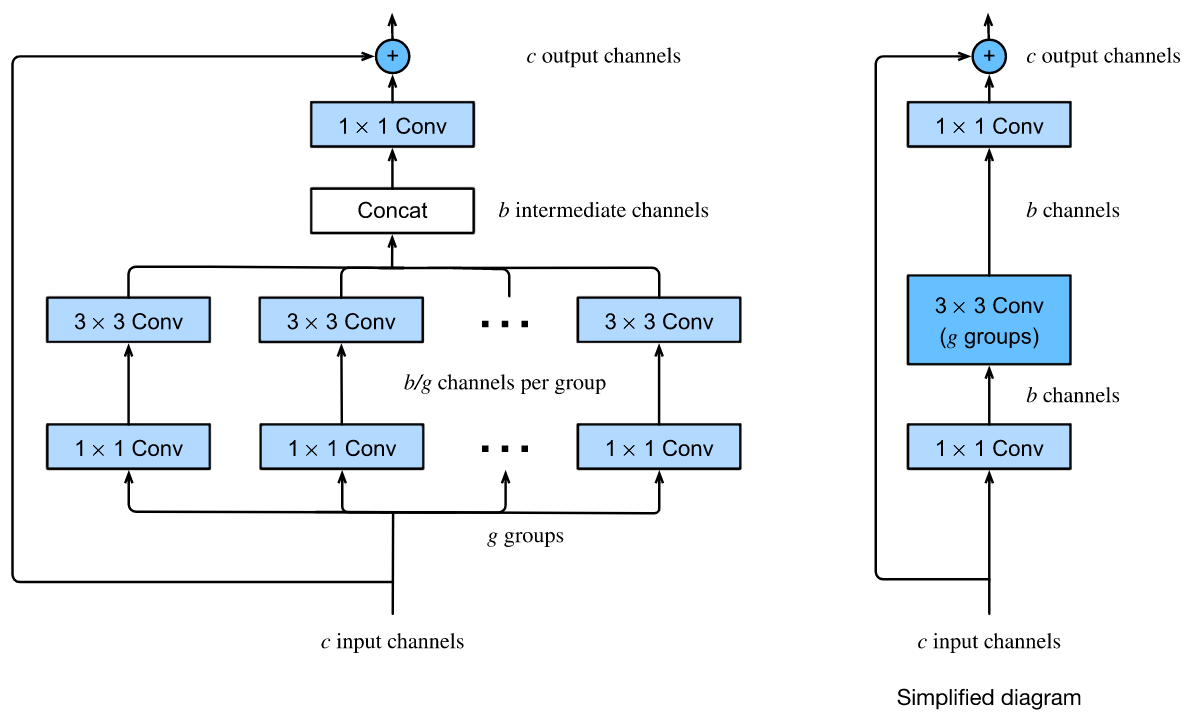
\includegraphics[width=0.8\columnwidth]{images/resnext.png}
    \caption{\cite{zhang2021dive}}
\end{figure}}


\frame{\frametitle{Final Notes}
\centering
\vspace{50 pt}
\textbf{Thank You!}
\vspace{50pt}

\textbf{Any Question?}
}


\frame{\frametitle{Refrences}
% \begin{itemize}
%     \printbibliography
% \end{itemize}
\bibliographystyle{plain}
\bibliography{Refrences}
}

%%%%%%%%%%%%%%%%%%%%%%%%%%%%%%%%%%%%%%%%%%
\end{document}